\documentclass[extendedabs]{bmvc2k}
\usepackage[ruled]{algorithm2e}
\begin{document}

\section*{digital image processing hw2}
\subsection*{problem 1: guided filter}

Guided filter \cite{guided} is an explicit image filter which have the edge-preserving 
smoothing property like the bilateral filter, but also handles gradient reversal artifacts.
In guided filter, filter output is assumed to be a linear transformation of guidance $I$
with linear coefficients $a_k$, $b_k$ in a window $\omega_k$ of center pixel $k$.
Coefficients are optimized to minimize the difference between $q$ and input $p$:
\[E(a_k,b_k) = \sum_{i \in \omega_k}((a_kI_i + b_k - p_i)^2 + \epsilon a_k^2)\]
\[a_k=\frac{1/|\omega|\sum_{i \in \omega_k}I_ip_i - \mu_k\bar{p_k}}{\sigma_k^2+\epsilon}\]
\[b_k=\bar{p_k} - a_k\mu_k\]
where $\mu_k$, $\sigma_k^2$ are the mean, variance of $I$ in $\omega_k$, 
$\bar{p_k}=1/|\omega|\sum_{i \in \omega_k}p_i$. 

When applying the window in the image, several windows $\omega_k$ can affect a same pixel.
Thus output $q$ can be averaged from all the possible windows:
\[q_i = 1/|\omega|\sum(a_kI_i + b_k)\]
The output can be also defined as a linear transformation of the input.
\[q_i = \sum_{j}W_ij(I)p_j\]
\[W_ij(I) = 1/|\omega|^2\sum_{k:(i,j) \in \omega_k}(1 + \frac{(I_i - \mu_k)(I_j - \mu_k)}{\sigma_k^2 + \epsilon})\]

Gradient preserving property can be found in \figurename{\ref{fig:1}}.
\begin{figure}[h]
    \centering
    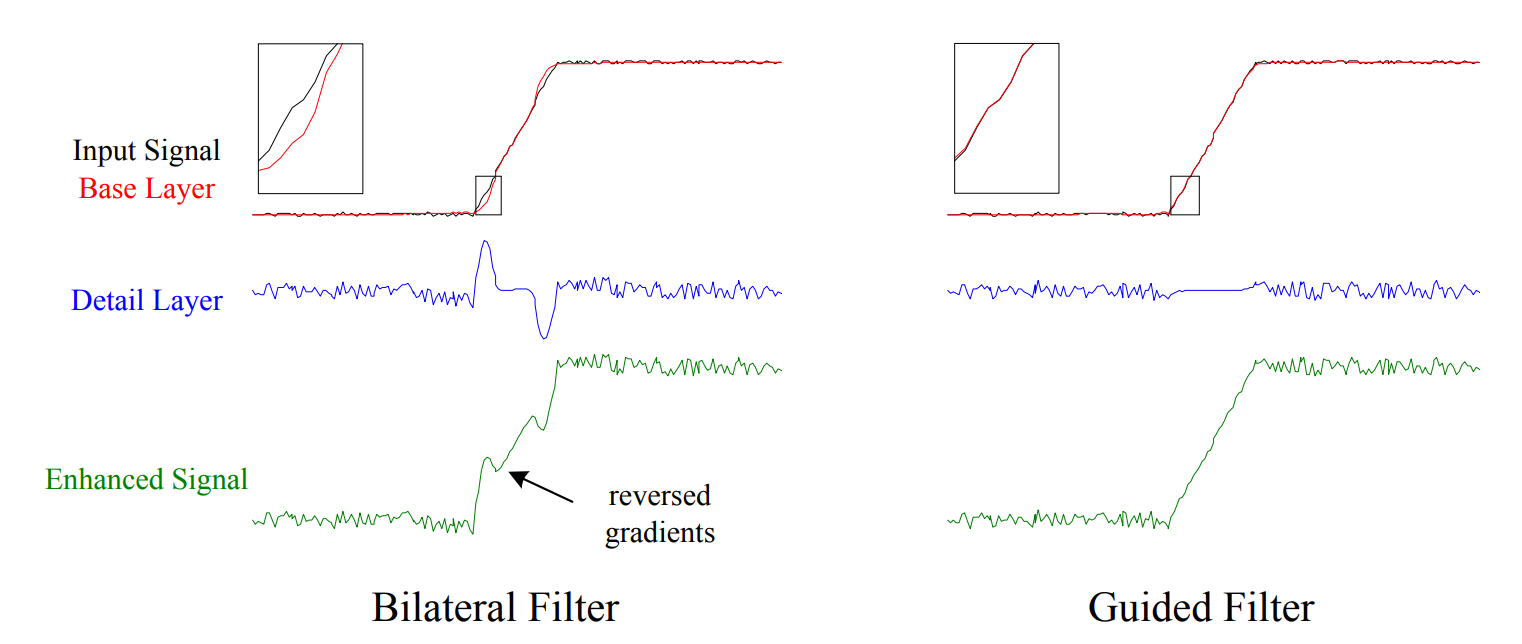
\includegraphics[width=\linewidth]{hw2_1_1}
    \caption{gradient reversal effect from bilateral filter and the corresponding guided filter result}
    \label{fig:1}
\end{figure}

\subsection*{problem 1: rolling guidance filter}

Rolling guidance filter \cite{rolling} is a scale-aware local operation filter that controls smoothing
details with a scale measure, by which small-scale structures can be removed while preserving others.
Rolling guidance filter consists of two steps; small structure removal and edge recovery.
At beginning, gaussian filter is used to remove small structures, which also involves blurring at
large-scale intensity variations.
\[G(p) = 1/K_p\sum_{q \in N(p)}exp(-\frac{||p-q||^2}{2\sigma_s^2})I(q)\]
\[K_p = \sum_{q \in N(p)}exp(-\frac{||p-q||^2}{2\sigma_s^2})\]
The next edge recovery step iteratively recovers edge with joint bilateral filter, with the guidance
image as its previous step output. $J^t$ stands for the recovery result from the $t$-th iteration.
\[J^{t+1}(p) = 1/K_p\sum_{q \in N(p)}exp(-\frac{||p-q||^2}{2\sigma_s^2}-\frac{||J^t(p)-J^t(q)||^2}{2\sigma_r^2})I(q)\]
\[K_p = \sum_{q \in N(p)}exp(-\frac{||p-q||^2}{2\sigma_s^2}-\frac{||J^t(p)-J^t(q)||^2}{2\sigma_r^2})\]
These two steps can be merged if $J^0$ is a constant-value image. Assign $J^t$ as a constant $C$, then
the resulting $J^t$ has the form exactly same as gaussian filter.

\begin{algorithm}
\caption{rolling guidance filter}
    $J^0 \gets$ constant image\;
    \For{$t = 1:num\_iter$}{
        $J^t \gets joint\_bilateral(I, J^{t-1}, \sigma_s, \sigma_r)$\;
    }
    return $J^{num\_iter}$\;
\end{algorithm}

\subsection*{problem 2: cross image filtering}

blah

\subsection*{problem 3: texture removal}

blah

\subsection*{problem 4: WLS filter}

blah

\subsection*{references}

\begin{thebibliography}{9}
    \bibitem{guided}
    K. He, J. Sun, and X. Tang, Guided Image Filtering, ECCV 2010.
    
    \bibitem{rolling}
    Q. Zhang et al., Rolling Guidance Filter, ECCV 2014.
\end{thebibliography}

\end{document}
